\documentclass[12]{scrartcl}
\usepackage{amssymb,amsmath,gensymb,dsfont,calc,multicol,fullpage,tikz}
\makeatletter
\newcommand\Aboxed[1]{
   \@Aboxed#1\ENDDNE}
\def\@Aboxed#1&#2\ENDDNE{%
   &
   \settowidth\@tempdima{$\displaystyle#1{}$}
   \setlength\@tempdima{\@tempdima+\fboxsep+\fboxrule}
   \kern-\@tempdima
   \boxed{#1#2}
}
\makeatother
\def\firstcircle{(90:1.75cm) circle (2.5cm)}
\def\secondcircle{(210:1.75cm) circle (2.5cm)}
\def\thirdcircle{(330:1.75cm) circle (2.5cm)}
\begin{document}
\title{Homework 13, Section  3.1: 2, 6, 9, 15, 18, 28}
\author{Alex Gordon}
\date{\today}
\maketitle
\section*{Homework}
\subsection*{2. A)}
4, 8, 12, 16, 20
\subsection*{2. B)}
4, 16, 36, 64, 100
\subsection*{2. C)}
4, 16, 36, 64, 100
\subsection*{2. D)}
4, 8 , 12, 16, 20
\subsection*{6. A)}
F
\subsection*{6. B)}
D
\subsection*{6. C)}
E
\subsection*{6. D)}
B
\subsection*{9. A)}
B
\subsection*{9. B)}
C
\subsection*{9. C)}
A
\subsection*{15. A)}
[1, 3, 5]
\subsection*{15. B)}
[1, 2, 3, 5]
\subsection*{15. C)}
[6, 7, 8, 9, 10]
\subsection*{15. D)}
[2, 4, 5, 6, 7, 8, 9, 10]
\subsection*{15. E)}
[1, 3, 5]
\subsection*{15. F)}
[1, 3, 5]
\subsection*{18. A)}
[$6x$ \textbar \ $x$ in $\mathds{Z}]$
\subsection*{18. B)}
[$2x$ \textbar \ $x$ in  $\mathds{Z}$ and $x$ $\neq$ 0 mod 6 ]
\subsection*{18. C)}
[$3y$ \textbar \ $y$ in  $\mathds{Z}$ and $y$ $\neq$ 0 mod 6 ]
\subsection*{18. D)}
[$x$ \textbar \ $x$ $0$ mod 2]
\subsection*{18. E)}
[$x$ \textbar \ $\mathds{Z}$ and $x$ $\neq$ $0$ mod 2]
\subsection*{28. A)}
    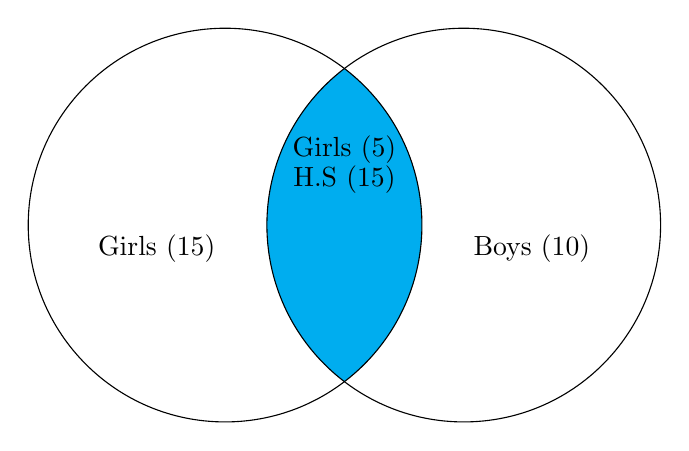
\begin{tikzpicture}
      \begin{scope}
    \clip \secondcircle;
    \fill[cyan] \thirdcircle;
      \end{scope}
      \begin{scope}
    \clip \secondcircle;
    \fill[cyan] \thirdcircle;
      \end{scope}
      \draw \secondcircle node [text=black,below left] {Girls (15)};
      \draw \thirdcircle node [text=black,below right] {Boys (10)};
      \draw node [text=black,below] {H.S (15)};
      \draw node [text=black,anchor=base] {Girls (5)};
    \end{tikzpicture}
\subsection*{28. B)}
    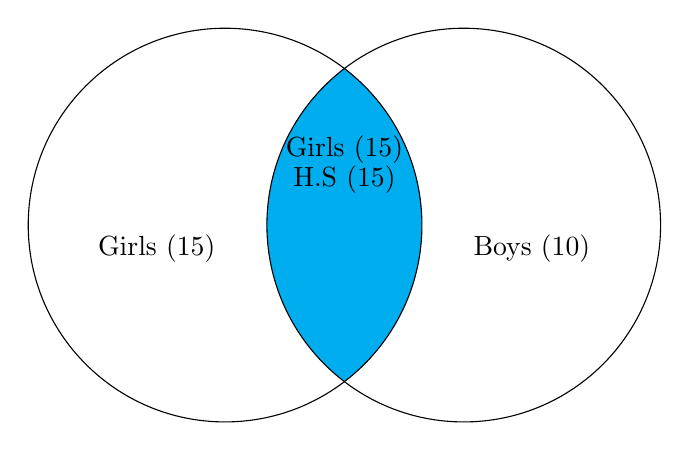
\begin{tikzpicture}
      \begin{scope}
    \clip \secondcircle;
    \fill[cyan] \thirdcircle;
      \end{scope}
      \begin{scope}
    \clip \secondcircle;
    \fill[cyan] \thirdcircle;
      \end{scope}
      \draw \secondcircle node [text=black,below left] {Girls (15)};
      \draw \thirdcircle node [text=black,below right] {Boys (10)};
      \draw node [text=black,below] {H.S (15)};
      \draw node [text=black,anchor=base] {Girls (15)};
    \end{tikzpicture}
\end{document}